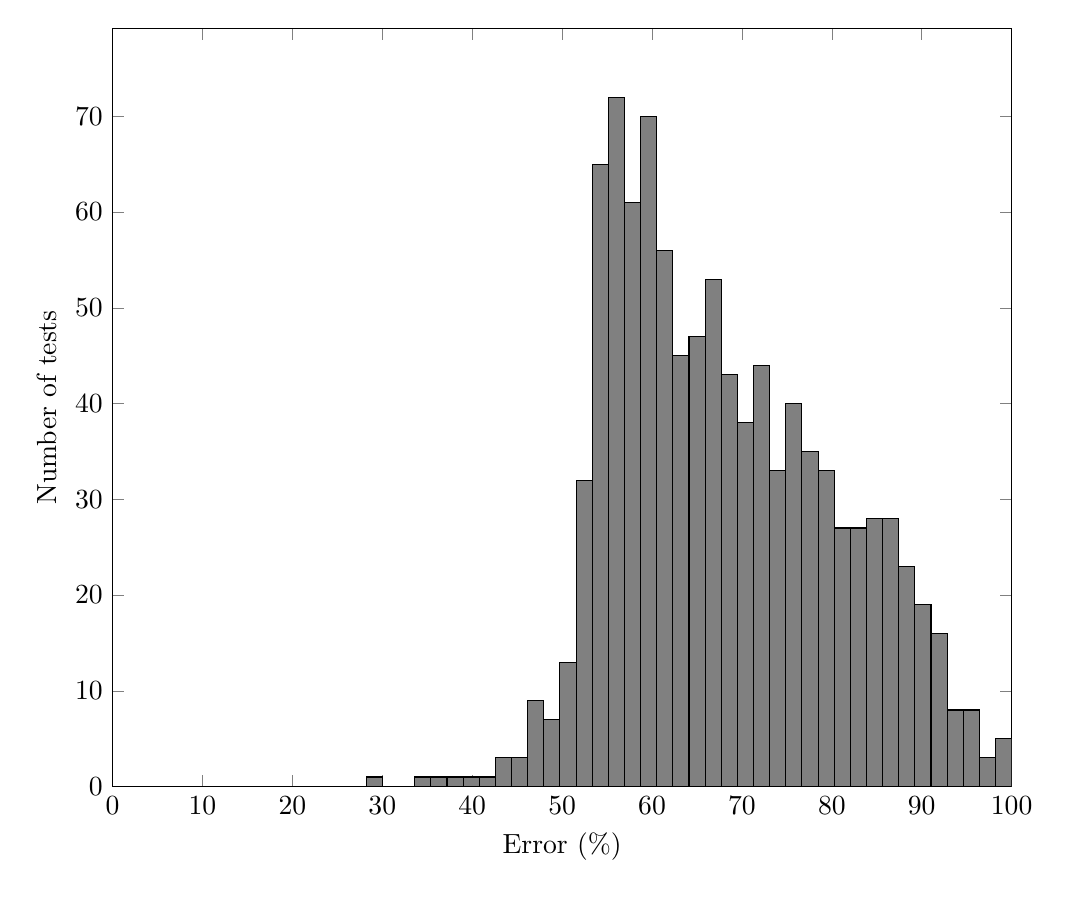
\begin{tikzpicture}
  \begin{axis}[
    width=13cm,
    ylabel=Number of tests,
    xlabel=Error (\%),
    xmin=0,xmax=100,ymin=0,]
    \addplot [ybar interval,fill=gray,draw=black] coordinates {
(28.22526783,  1.)
(30.01963612,  0.)
(31.81400442,  0.)
(33.60837272,  1.)
(35.40274101,  1.)
(37.19710931,  1.)
(38.9914776, 1.)
(40.7858459, 1.)
(42.58021419,  3.)
(44.37458249,  3.)
(46.16895078,  9.)
(47.96331908,  7.)
(49.75768737, 13.)
(51.55205567, 32.)
(53.34642397, 65.)
(55.14079226, 72.)
(56.93516056, 61.)
(58.72952885, 70.)
(60.52389715, 56.)
(62.31826544, 45.)
(64.11263374, 47.)
(65.90700203, 53.)
(67.70137033, 43.)
(69.49573862, 38.)
(71.29010692, 44.)
(73.08447522, 33.)
(74.87884351, 40.)
(76.67321181, 35.)
(78.4675801,  33.)
(80.2619484,  27.)
(82.05631669, 27.)
(83.85068499, 28.)
(85.64505328, 28.)
(87.43942158, 23.)
(89.23378987, 19.)
(91.02815817, 16.)
(92.82252647,  8.)
(94.61689476,  8.)
(96.41126306,  3.)
(98.20563135,  5.)
(99.99999965,  0.)
    };
  \end{axis}
\end{tikzpicture}